\documentclass[../main.tex]{subfiles}
\graphicspath{{\subfix{../images/}}}
\begin{document}

\section{Methodology}

\subsection{Network architecture}

\begin{figure}[h!]
  \centering
  \begin{subfigure}[b]{\linewidth}
    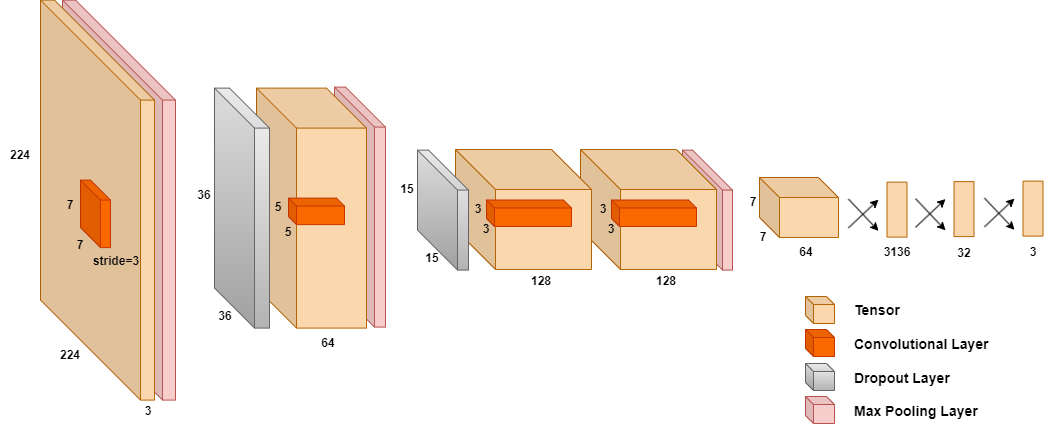
\includegraphics[width=\linewidth]{NetworkDiagram.drawio.png}
    \caption{Diagram of the Network}
  \end{subfigure}
  \label{fig:network-diagram}
\end{figure}

The model contains 5 convolution layers and 3 fully connected classification layers. 

The kernels of the first layer is 7 pixels in height and width with a stride of 3, extracting 64 layers. The overlapping max pooling layer is then added with kernel size 3 and stride 2.

A dropout layer with drop probability of 50\% is added before the second convolutional layer with size 5 kernel extracting 128 feature into a max pooling layer. 

Another dropout layer is added for the 3rd set of convolution layers. The inputs then go through 2 sets of convolution layers with kernel size 3. The first of the set extracts 128 layers and the second extracts 64 layers. The output is put through the final max pooling layer. 

The output will be flatten and inputted into 3 classification layers with 3136 input nodes, 32 hidden nodes and 3 output nodes representing each fruit class. 

This model was adapted from the AlexNet model and utilised several of its key features. The use of overlapping pooling layers which was found to reduce overfitting slightly. Another way overfitting was avoided was through the use of the dropout layer that randomly dropped nodes from the output with a 50\% probability, forcing the network to find alternative features which reduces the weights given to any singular feature. 

\subsection{Pre-Processing}

During training, random augments of the images were performed onto the images to diversify our dataset. By diversifying the dataset, the model will be trained to identify patterns in the data and from that learn to identify fruit in unmodified images. 

Following the changes, the images are then resized to 256 pixels in height and width before cropping a 224 pixel square in the middle. This allows the model to focus on the middle of the image without noticing any noise that may exist in the background. 

Finally, the image is converted to a tensor and every value is normalised by mapping each value to a value in a normal distribution with a mean of 0.5 and standard deviation of 0.5.

The pre processing steps are performed on the validation and testing images as well except the random augments are removed. 

\subsection{Optimisation Function}

The chosen optimisation function was the Stochastic Gradient Descent (SGD) function, this function was chosen as the Adam function failed to improve from the model's initialisation.

\subsection{Loss Function}

The loss function selected for this model was the NLLLoss because through testing found that it improved the accuracy of the model by 10\%. 

\subsection{Activation Function}

The use of the ReLU function was used at each layer except for the output layer. The ReLU function was used as it reduced the error of the network in fewer iterations than other activation functions. The output layer used the SoftMax function as required by the NLLLoss function. 

\subsection{Batch Size and Learning Rate}

It was determined that lower batch sizes were beneficial due to less of a need to compensate for the lack of updates by increasing the learning rate. The increase in learning rate caused greater changes to the accuracy which can cause the model not to converge. 

\subsection{Epochs}
With the given parameters, the model converged to an accuracy of 80\% on the validation set within 68 epochs. 

\end{document}